\chapter{Polymeren}\label{ch:g12:polymers}

Een fleecevest kan gesponnen worden uit gesmolten drankflessen; een
klimtouw is van nylon gemaakt; deze bladzijde is cellulose, gemaakt door
bomen. Alle drie zijn het \omterm{def:g12:polymers:polymer}{polymeren}: \omterm{def:g7:atoms-and-molecules:molecule}{moleculen} van duizenden \omterm{def:g7:atoms-and-molecules:atom}{atomen} lang,
opgebouwd door één kleine eenheid steeds weer te herhalen. Hun
eigenschappen --- zacht of stijf, elastisch of bros, smeltbaar of niet ---
komen minder voort uit de \omterm{def:g7:atoms-and-molecules:atom}{atomen} die ze bevatten dan uit de manier
waarop hun lange ketens gerangschikt zijn.

\begin{recall}
\omterm{def:g8:plastics:plastic}{Kunststoffen} bestaan uit heel lange \omterm{def:g7:atoms-and-molecules:molecule}{moleculen}; \omterm{def:g8:plastics:thermoplastic}{thermoplasten} worden zacht
bij verwarmen, \omterm{def:g8:plastics:thermoplastic}{thermoharders} niet (\cref{ch:g8:plastics}). Alcohol-,
zuur-, ester-, amine- en amidegroepen (\cref{ch:g11:functional-groups}).
Een additie maakt van twee \omterm{def:g7:atoms-and-molecules:molecule}{moleculen} één, zonder dat er een \omterm{def:g7:atoms-and-molecules:atom}{atoom}
verloren gaat
(\cref{ch:g12:curly-arrows}).
\end{recall}

\begin{omfigure}
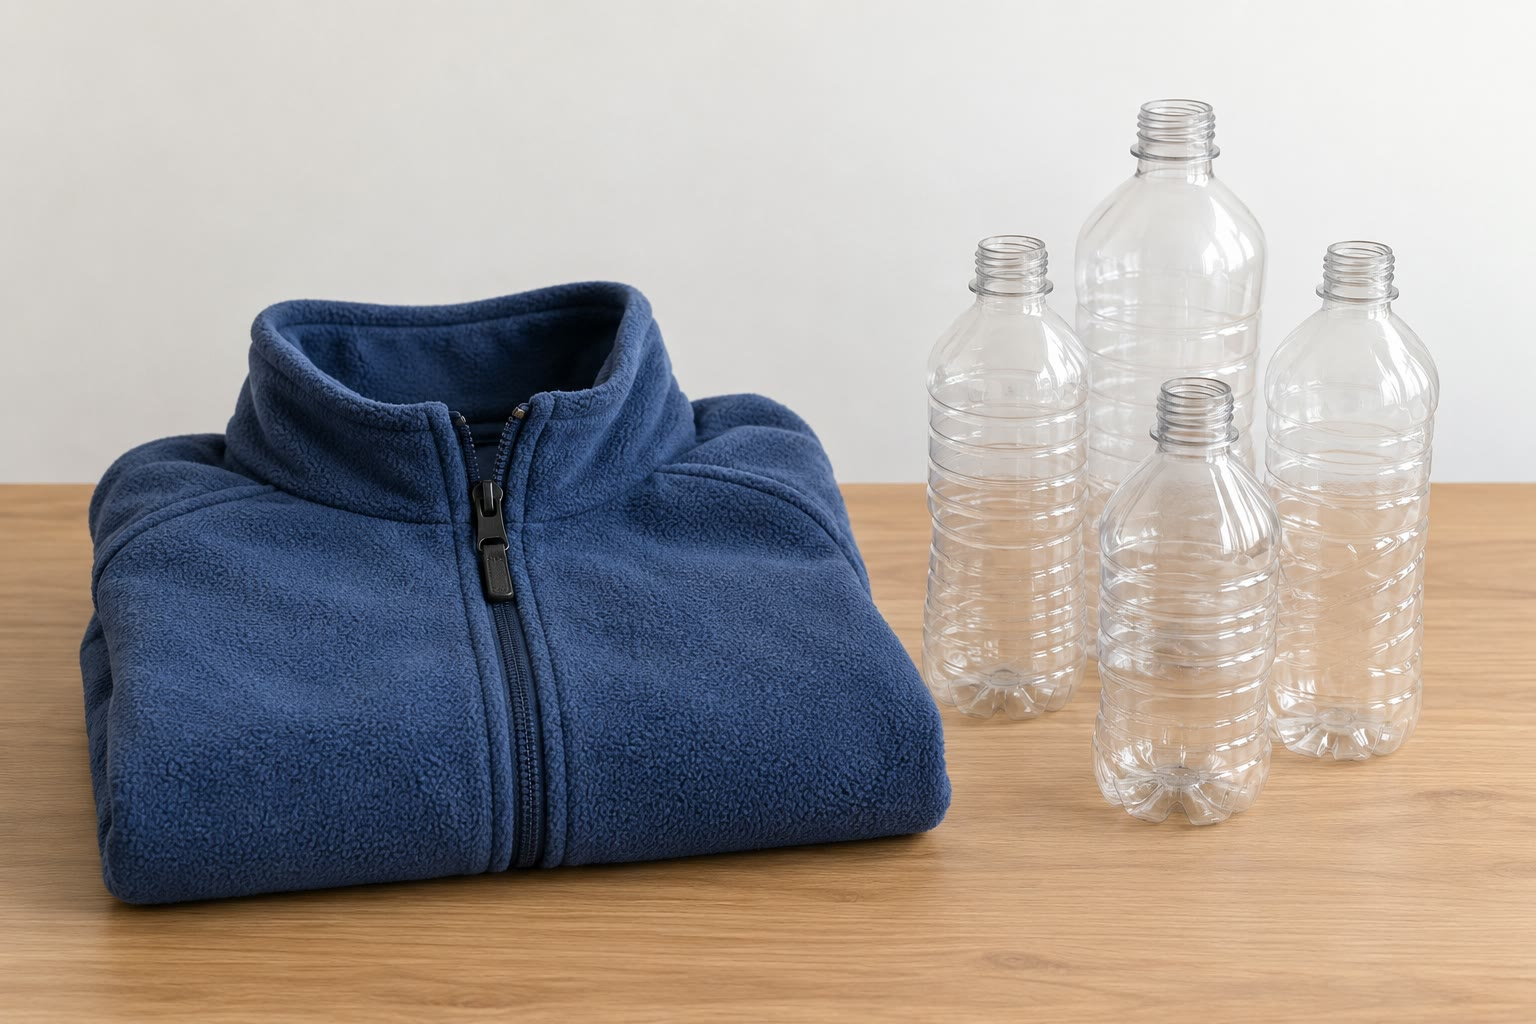
\includegraphics[width=0.45\linewidth]{images/book1/ai/g12-fleece-bottles.jpg}

{\small Gebruikte drankflessen en een fleecevest: hetzelfde \omterm{def:g12:polymers:polymer}{polymeer}, in
twee vormen.}
\end{omfigure}

\section{Monomeren, polymeren, repeterende eenheden}

\begin{definition}[Polymeer, monomeer, polymerisatie]\label{def:g12:polymers:polymer}
Een \emph{polymeer}\index{polymeer} is een stof die bestaat uit heel grote
\omterm{def:g7:atoms-and-molecules:molecule}{moleculen}, de macromoleculen, elk opgebouwd uit veel kleine eenheden die
een voor een aan elkaar gebonden zijn. De kleine \omterm{def:g7:atoms-and-molecules:molecule}{moleculen} waaruit het
gemaakt wordt, zijn zijn \emph{monomeren}\index{monomeer}; de reactie die
ze aan elkaar koppelt, is een
\emph{polymerisatie}\index{polymerisatie}.
\end{definition}

\begin{definition}[Repeterende eenheid, polymerisatiegraad]\label{def:g12:polymers:repeat-unit}
De \emph{repeterende eenheid}\index{repeterende eenheid} van een \omterm{def:g12:polymers:polymer}{polymeer}
is de kleinste groep \omterm{def:g7:atoms-and-molecules:atom}{atomen} waarvan de herhaling de keten geeft; ze wordt
tussen haken geschreven met een \omterm{def:g7:atoms-and-molecules:formula}{index} $n$. Het aantal $n$ repeterende
eenheden in een keten is de
\emph{polymerisatiegraad}\index{polymerisatiegraad} ervan.
\end{definition}

\begin{omfigure}
\[
  n\;\ce{CH2=CH2}
  \quad\longrightarrow\quad
  \chemfig{-[@{op1,.75}]CH_2-CH_2-[@{cl1,0.25}]}
  \polymerdelim[height=6pt, depth=6pt, indice=n]{op1}{cl1}
\]

{\small De \omterm{def:g12:polymers:polymer}{polymerisatie} van etheen: $n$ \omterm{def:g7:atoms-and-molecules:molecule}{moleculen} \omterm{def:g12:polymers:polymer}{monomeer} geven één
keten polyetheen, waarvan de \omterm{def:g12:polymers:repeat-unit}{repeterende eenheid} \ce{-CH2-CH2-} tussen
haken wordt geschreven.}
\end{omfigure}

\begin{proposition}[Molaire massa van een polymeer]\label{prop:g12:polymers:molar-mass}
Een keten met \omterm{def:g12:polymers:repeat-unit}{polymerisatiegraad} $n$ heeft een \omterm{def:g10:the-mole:molar-mass}{molaire massa}
\[
  M(\text{polymeer}) \approx n \times M(\text{repeterende eenheid}) ,
\]
waarbij de twee uiteinden van de keten bij grote $n$ te verwaarlozen zijn.
\end{proposition}

\begin{proof}
De keten bestaat uit $n$ \omterm{def:g12:polymers:repeat-unit}{repeterende eenheden} plus twee eindgroepen van
elk een paar \omterm{def:g7:atoms-and-molecules:atom}{atomen}; bij $n$ in de duizenden wegen de eindgroepen minder
dan een duizendste van het geheel.
\end{proof}

\begin{example}[Een keten polyetheen]\label{ex:g12:polymers:pe}
% ledger: aw:C, aw:H
Een keten polyetheen met een \omterm{def:g10:the-mole:molar-mass}{molaire massa} van \qty{280000}{g/mol} heeft
$n = 280000/28.0 = 10000$ \omterm{def:g12:polymers:repeat-unit}{repeterende eenheden}, dus twintigduizend
koolstofatomen op een rij. In een echt monster zijn de ketens niet
allemaal even lang:
$n$ is een gemiddelde.
\end{example}

\section{Additiepolymeren}

\begin{definition}[Additiepolymeer, condensatiepolymeer]\label{def:g12:polymers:addition-polymer}
Een \emph{additiepolymeer}\index{additiepolymeer} ontstaat door additie
van \omterm{def:g12:polymers:polymer}{monomeren} met een \omterm{def:g10:lewis-and-shape:multiple-bond}{dubbele binding} \ce{C=C}, zonder ander product: zijn
\omterm{def:g12:polymers:repeat-unit}{repeterende eenheid} bevat dezelfde \omterm{def:g7:atoms-and-molecules:atom}{atomen} als het \omterm{def:g12:polymers:polymer}{monomeer}. Een
\emph{condensatiepolymeer}\index{condensatiepolymeer} ontstaat door
reacties tussen twee \omterm{def:g11:functional-groups:functional-group}{karakteristieke groepen} die twee \omterm{def:g12:polymers:polymer}{monomeren} aan elkaar
koppelen en bij elke koppeling een klein \omterm{def:g7:atoms-and-molecules:molecule}{molecuul} afsplitsen, meestal
water.
\end{definition}

\begin{omfigure}
\footnotesize
\renewcommand{\arraystretch}{1.5}
\begin{tabular}{l l l l}
\hline
\omterm{def:g12:polymers:polymer}{monomeer} & \omterm{def:g12:polymers:polymer}{polymeer} & \omterm{def:g12:polymers:repeat-unit}{repeterende eenheid} & toepassingen \\
\hline
etheen \ce{CH2=CH2} & polyetheen (PE) & \ce{-CH2-CH2-} & tassen, flessen \\
chlooretheen \ce{CH2=CHCl} & polyvinylchloride (PVC) & \ce{-CH2-CHCl-} & buizen, kozijnen \\
fenyletheen \ce{CH2=CH-C6H5} & polystyreen (PS) & \ce{-CH2-CH(C6H5)-} & bekers, schuim \\
tetrafluoretheen \ce{CF2=CF2} & PTFE & \ce{-CF2-CF2-} & antiaanbakpannen \\
\hline
\end{tabular}\par\medskip

{\small Vier \omterm{def:g12:polymers:addition-polymer}{additiepolymeren}. In elk ervan klapt de \omterm{def:g10:lewis-and-shape:multiple-bond}{dubbele binding} van
het \omterm{def:g12:polymers:polymer}{monomeer} open, en worden de twee koolstofatomen deel van de keten.}
\end{omfigure}

\begin{method}[Het monomeer vinden bij een polymeer]\label{met:g12:polymers:monomer}
\begin{enumerate}
  \item Zoek de \omterm{def:g12:polymers:repeat-unit}{repeterende eenheid}: de kleinste groep waarvan de
        herhaling de keten geeft.
  \item Als de hoofdketen alleen koolstofatomen bevat, is het een
        \omterm{def:g12:polymers:addition-polymer}{additiepolymeer}: zet een \omterm{def:g10:lewis-and-shape:multiple-bond}{dubbele binding} terug tussen de twee
        koolstofatomen van de hoofdketen van de \omterm{def:g12:polymers:repeat-unit}{repeterende eenheid}. Dat
        is het \omterm{def:g12:polymers:polymer}{monomeer}.
  \item Als de hoofdketen ester- of amidebindingen bevat, is het een
        \omterm{def:g12:polymers:addition-polymer}{condensatiepolymeer}: knip elke binding door, en geef elke kant de
        \omterm{def:g7:atoms-and-molecules:atom}{atomen} van het afgesplitste kleine \omterm{def:g7:atoms-and-molecules:molecule}{molecuul} terug (\ce{-OH} aan de
        \ce{C=O}, \ce{-H} aan de \ce{O} of de \ce{N}). Dat zijn de
        \omterm{def:g12:polymers:polymer}{monomeren}.
\end{enumerate}
\end{method}

\begin{example}[Het monomeer van PVC]\label{ex:g12:polymers:pvc}
De keten \ce{-CH2-CHCl-CH2-CHCl-CH2-CHCl-} herhaalt \ce{-CH2-CHCl-}; de
hoofdketen bevat alleen koolstofatomen, dus het \omterm{def:g12:polymers:polymer}{monomeer} is
chloor\-etheen, \ce{CH2=CHCl}.
\end{example}

\section{Condensatiepolymeren}

Een \omterm{def:g12:polymers:polymer}{monomeer} met één reactieve groep kan maar één keer binden: het sluit
een keten af. Om een keten door condensatie op te bouwen, heeft elk
\omterm{def:g12:polymers:polymer}{monomeer} twee groepen nodig, één aan elk uiteinde.

\begin{example}[PET, een polyester]\label{ex:g12:polymers:pet}
% ledger: aw:C, aw:H, aw:O
Ethaan-1,2-diol, \ce{HO-CH2-CH2-OH}, draagt twee alcoholgroepen;
benzeen-1,4-dicarbonzuur, \ce{HOOC-C6H4-COOH}, twee zuurgroepen. Elke
zuurgroep vormt een \omterm{def:g11:functional-groups:carboxylic-acid}{ester} met een alcoholgroep en splitst water af: de
keten groeit aan beide uiteinden. Het \omterm{def:g12:polymers:polymer}{polymeer} is
polyethyleentereftalaat, PET, het materiaal van drankflessen en van
polyestervezels. Zijn \omterm{def:g12:polymers:repeat-unit}{repeterende eenheid}, \ce{C10H8O4}, heeft een \omterm{def:g10:the-mole:molar-mass}{molaire
massa} van \qty{192.0}{g/mol}, dat is de twee \omterm{def:g12:polymers:polymer}{monomeren}
($62.0 + 166.0$) min twee \omterm{def:g7:atoms-and-molecules:molecule}{moleculen} water ($36.0$).
\end{example}

\begin{omfigure}
\setchemfig{atom sep=1.9em}
\chemfig{HO-CH_2-CH_2-OH}
\quad $+$ \quad
\chemfig{HO-C(=[2]O)-*6(-=-(-C(=[2]O)-OH)=-=)}

\medskip
$\longrightarrow$\quad
\chemfig{-[@{op2,.75}]O-CH_2-CH_2-O-C(=[2]O)-*6(-=-(-C(=[2]O)-[@{cl2,0.25}])=-=)}
\polymerdelim[height=20pt, depth=6pt, indice=n]{op2}{cl2}
\quad $+\ 2n\ \ce{H2O}$

{\small PET uit zijn twee \omterm{def:g12:polymers:polymer}{monomeren}: elke esterbinding (de
\ce{-CO-O-}-groepen) splitst één \omterm{def:g7:atoms-and-molecules:molecule}{molecuul} water af.}
\end{omfigure}

\begin{example}[Nylon-6,6, een polyamide]\label{ex:g12:polymers:nylon}
Hexaan-1,6-diamine, \ce{H2N-(CH2)6-NH2}, en hexaandizuur,
\ce{HOOC-(CH2)4-COOH}, worden door amidebindingen aan elkaar gekoppeld,
die elk één \omterm{def:g7:atoms-and-molecules:molecule}{molecuul} water afsplitsen:
\[
  \cdots\ce{-NH-(CH2)6-NH-CO-(CH2)4-CO-}\cdots
\]
De twee zessen in de naam tellen de koolstofatomen van elk \omterm{def:g12:polymers:polymer}{monomeer}. De
amidebindingen van naburige ketens trekken elkaar aan via
\omterm{def:g11:polarity-and-cohesion:hydrogen-bond}{waterstofbruggen}, wat nylonvezels sterk maakt.
\end{example}

\begin{history}[Carothers en nylon]
% ledger: hist:polyamides-1934, hist:nylon-production-1939
De scheikundige Wallace Carothers, die een onderzoekslaboratorium van een
chemisch bedrijf leidde, wilde bewijzen dat \omterm{def:g12:polymers:polymer}{polymeren} echte reuzenmoleculen
waren, en ze doelbewust maken. Zijn team maakte eerst polyesters, die te
gemakkelijk smolten om bruikbaar te zijn; in 1934 stapten ze over op
\omterm{def:g11:functional-groups:amine}{aminen} en maakten ze polyamiden, waaronder de vezel die later nylon werd
genoemd. Nylon ging in 1939 in productie, eerst als kousen die op een
wereldtentoonstelling opzien baarden, daarna als parachutes, touwen en
tandenborstelharen.
\end{history}

\begin{omfigure}
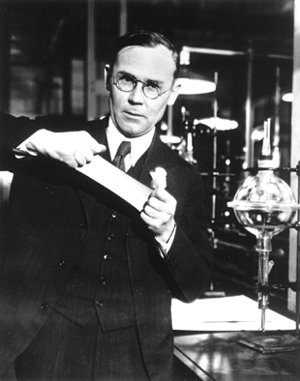
\includegraphics[width=0.24\linewidth]{images/book1/carothers.jpg}

{\small Wallace Carothers in zijn laboratorium.}
\end{omfigure}

\section{Structuur en eigenschappen}

Twee monsters van hetzelfde \omterm{def:g12:polymers:polymer}{polymeer} kunnen zich heel verschillend
gedragen: het gaat om de lengte van de ketens, hun vorm, en hoe ze
gestapeld zijn.

\begin{proposition}[Ketens en eigenschappen]\label{prop:g12:polymers:properties}
\begin{itemize}
  \item Langere ketens raken meer verstrengeld: het materiaal is sterker
        en smelt bij een hogere temperatuur.
  \item Lineaire ketens kunnen naast elkaar komen te liggen in geordende,
        \emph{kristallijne} gebieden; vertakte ketens kunnen dat niet, en
        blijven ongeordend, \emph{amorf}. Kristallijne gebieden maken een
        \omterm{def:g12:polymers:polymer}{polymeer} dichter, stijver en minder doorzichtig.
  \item Ketens die alleen door intermoleculaire krachten naast elkaar
        worden gehouden, glijden bij verwarmen langs elkaar: het \omterm{def:g12:polymers:polymer}{polymeer}
        is een \omterm{def:g8:plastics:thermoplastic}{thermoplast}. Ketens die door covalente
        \emph{dwarsverbindingen} aan elkaar vastzitten, kunnen dat niet:
        het \omterm{def:g12:polymers:polymer}{polymeer} is een \omterm{def:g8:plastics:thermoplastic}{thermoharder}, of, met weinig
        dwarsverbindingen, een rubberachtige elastische vaste stof.
\end{itemize}
\end{proposition}

\begin{proof}
Verwarmen geeft de ketens genoeg energie om de intermoleculaire krachten
tussen hen te overwinnen (\cref{ch:g11:polarity-and-cohesion}), die
zwakker zijn dan \omterm{def:g10:lewis-and-shape:covalent-bond}{covalente bindingen}; hoe meer contact tussen de ketens,
hoe meer energie dat kost. Dwarsverbindingen zijn covalent: als je ze
verbreekt, vernietig je het materiaal in plaats van het te smelten.
\end{proof}

\begin{omfigure}
\begin{tikzpicture}[font=\footnotesize, line width=1pt, line cap=round,
    lab/.style={below, align=center, text width=2.8cm}]
  % lineair, gestapeld (kristallijn)
  \begin{scope}
    \foreach \y in {0,0.25,0.5,0.75,1.0}
      \draw[omDef] plot[smooth, domain=0:2.2, samples=25] (\x, {\y + 0.05*sin(400*\x)});
    \node[lab] at (1.1,-0.2) {lineaire ketens\\ op een rij: kristallijn};
  \end{scope}
  % lineair, verstrengeld (amorf)
  \begin{scope}[xshift=3.4cm]
    \draw[omDef] plot[smooth] coordinates {(0,0.2) (0.5,0.9) (1.0,0.3) (1.4,1.1) (2.0,0.5) (2.2,0.9)};
    \draw[omProp] plot[smooth] coordinates {(0,0.9) (0.4,0.3) (0.9,1.0) (1.5,0.2) (1.9,1.0) (2.2,0.3)};
    \draw[black!60] plot[smooth] coordinates {(0.1,0.55) (0.7,0.1) (1.2,0.75) (1.7,0.55) (2.2,0.1)};
    \node[lab] at (1.1,-0.2) {lineaire ketens\\ verstrengeld: amorf};
  \end{scope}
  % vertakt
  \begin{scope}[xshift=6.8cm]
    \draw[omDef] plot[smooth] coordinates {(0,0.5) (0.6,0.6) (1.2,0.45) (1.8,0.65) (2.2,0.5)};
    \draw[omDef] (0.5,0.6) -- (0.35,1.05) (1.0,0.5) -- (1.15,0.05) (1.6,0.6) -- (1.5,1.1) (1.6,0.6) -- (1.95,1.0);
    \node[lab] at (1.1,-0.2) {vertakte ketens:\\ stapelen niet};
  \end{scope}
  % met dwarsverbindingen
  \begin{scope}[xshift=10.2cm]
    \foreach \y in {0.1,0.55,1.0}
      \draw[omDef] plot[smooth, domain=0:2.2, samples=25] (\x, {\y + 0.06*sin(300*\x)});
    \foreach \x/\a/\b in {0.4/0.1/0.55, 1.3/0.1/0.55, 0.9/0.55/1.0, 1.9/0.55/1.0}
      \draw[omProp, line width=1.6pt] (\x,\a) -- (\x,\b);
    \node[lab] at (1.1,-0.2) {ketens met dwars-\\ verbindingen: smelten niet};
  \end{scope}
\end{tikzpicture}

{\small Vier rangschikkingen van polymeerketens. De dwarsverbindingen
(oranje) zijn \omterm{def:g10:lewis-and-shape:covalent-bond}{covalente bindingen} tussen ketens.}
\end{omfigure}

\begin{example}[Twee soorten polyetheen]\label{ex:g12:polymers:two-pe}
Polyetheen dat onder zeer hoge druk wordt gemaakt, heeft veel korte
zijtakken: de ketens stapelen slecht, en het levert zachte, doorzichtige
folie voor tassen. Gemaakt met een \omterm{def:g12:catalysis:catalyst}{katalysator} bij lage druk zijn de
ketens bijna lineair en stapelen ze tot kristallijne gebieden: het is
dichter en stijver, en levert melkflessen en kratten. Hetzelfde \omterm{def:g12:polymers:polymer}{monomeer},
dezelfde \omterm{def:g12:polymers:repeat-unit}{repeterende eenheid}, een andere architectuur.
\end{example}

\section{Natuurlijke polymeren}

Levende wezens maakten al \omterm{def:g12:polymers:polymer}{polymeren}, lang voordat scheikundigen dat
deden.

\begin{itemize}
  \item \textbf{Cellulose} en \textbf{zetmeel} zijn allebei ketens van
        glucose-eenheden, \ce{C6H10O5} per eenheid, die verschillend aan
        elkaar zijn gekoppeld: cellulose vormt rechte, sterke vezels
        (hout, katoen, papier); zetmeel vormt spiralen die het lichaam
        verteert.
  \item \textbf{Eiwitten} zijn ketens van aminozuren die door
        amidebindingen aan elkaar zijn gekoppeld, de peptidebindingen van
        het dipeptide van
        \cref{ch:g12:synthesis-strategy}.
  \item \textbf{DNA} is een keten van nucleotiden; de volgorde van zijn
        vier soorten eenheden slaat genetische informatie op.
  \item \textbf{Natuurrubber} is een \omterm{def:g12:polymers:addition-polymer}{additiepolymeer} van isopreen,
        \ce{CH2=C(CH3)-CH=CH2}, dat als een melkachtige vloeistof, latex,
        uit de bast van de rubberboom wordt gewonnen. Als je het met
        zwavel verwarmt, worden de ketens verbonden door zwavelbruggen: het
        rubber wordt taaier en houdt zijn vorm, zoals in een band.
\end{itemize}

\begin{omfigure}
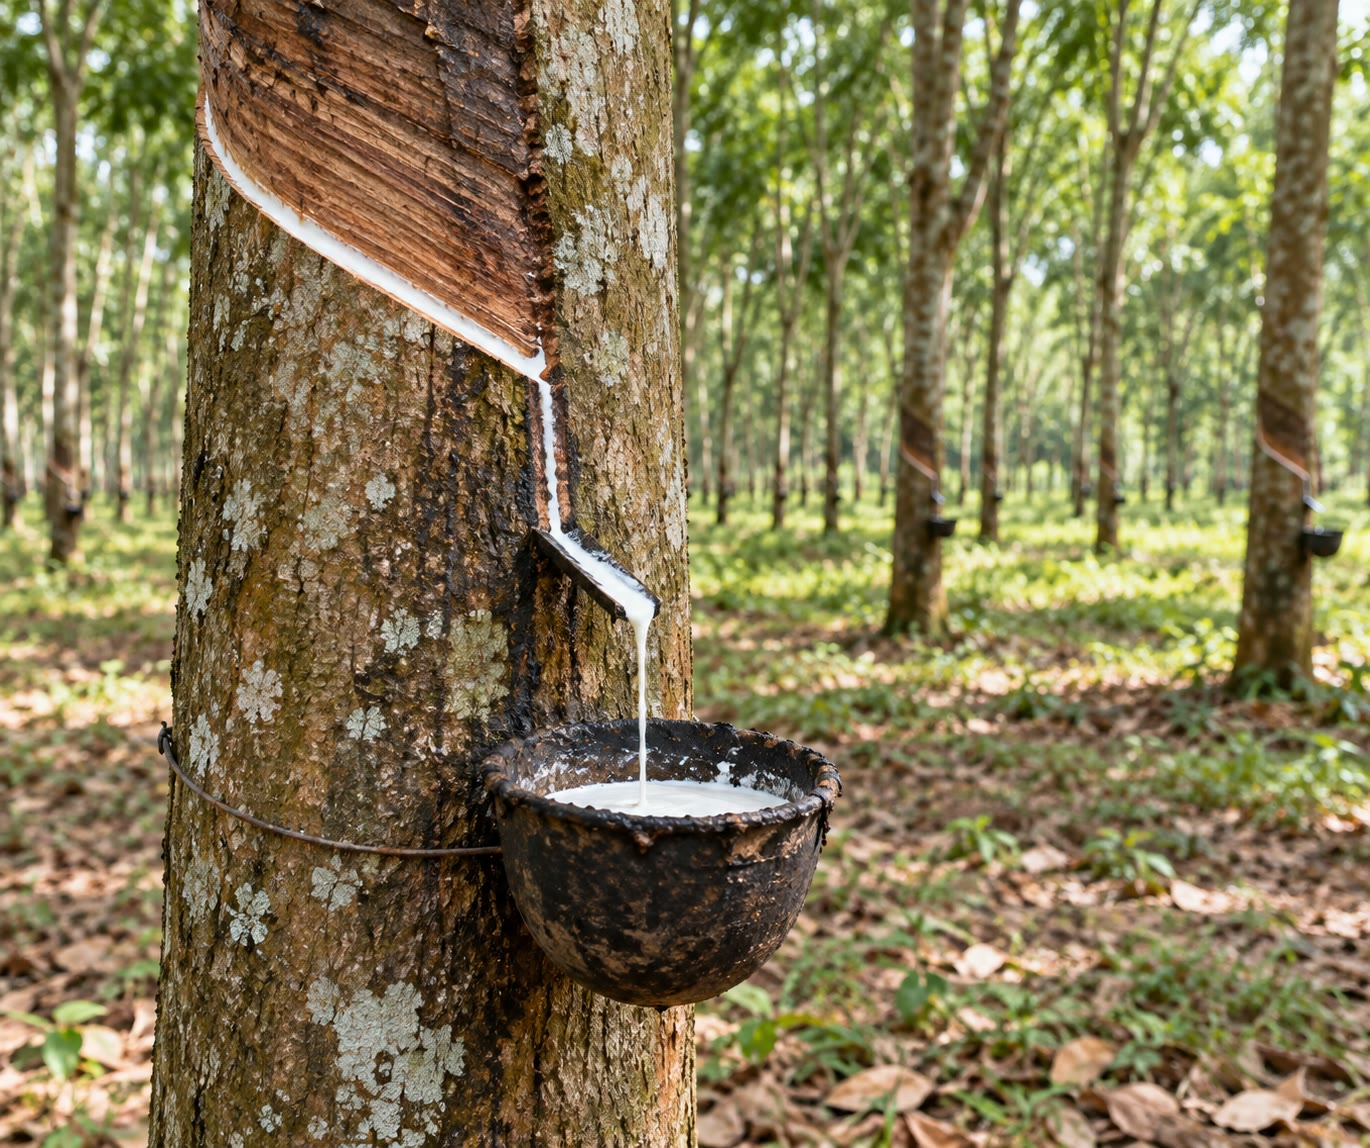
\includegraphics[width=0.45\linewidth]{images/book1/ai/g12-rubber-tapping.jpg}

{\small Een rubberboom tappen: latex stroomt uit een snee in de bast in
een bakje.}
\end{omfigure}

\begin{remark}[Maken en afbreken]\label{rem:g12:polymers:recycling}
Een \omterm{def:g8:plastics:thermoplastic}{thermoplast} kun je opnieuw smelten en vormen: mechanische \omterm{def:g5:raw-materials-and-recycling:recycling}{recycling}.
Een \omterm{def:g12:polymers:addition-polymer}{condensatiepolymeer} kun je ook terug afbreken tot zijn \omterm{def:g12:polymers:polymer}{monomeren} door
de omgekeerde reactie, een hydrolyse, en van die \omterm{def:g12:polymers:polymer}{monomeren} nieuw \omterm{def:g12:polymers:polymer}{polymeer}
maken: chemische \omterm{def:g5:raw-materials-and-recycling:recycling}{recycling}. Een \omterm{def:g8:plastics:thermoplastic}{thermoharder} kan geen van beide
gemakkelijk.
\end{remark}

\section{Oefeningen}

\begin{exercise}[$\star$]\label{exo:g12:polymers:1}
Geef het \omterm{def:g12:polymers:polymer}{monomeer} van polypropeen, waarvan de \omterm{def:g12:polymers:repeat-unit}{repeterende eenheid}
\ce{-CH2-CH(CH3)-} is.
\end{exercise}

\begin{exercise}[$\star$]\label{exo:g12:polymers:2}
Schrijf de \omterm{def:g12:polymers:repeat-unit}{repeterende eenheid} op van het \omterm{def:g12:polymers:polymer}{polymeer} dat uit
tetrafluoretheen,
\ce{CF2=CF2}, wordt gemaakt. Is het een additie- of een
\omterm{def:g12:polymers:addition-polymer}{condensatiepolymeer}?
\end{exercise}

\begin{exercise}[$\star$]\label{exo:g12:polymers:3}
Deel in bij de additie- of \omterm{def:g12:polymers:addition-polymer}{condensatiepolymeren}: polyetheen, PET, nylon,
PVC, polystyreen.
\end{exercise}

\begin{exercise}[$\star$]\label{exo:g12:polymers:4}
Welke van deze \omterm{def:g12:polymers:polymer}{polymeren} zijn natuurlijk: cellulose, nylon, zetmeel, PVC,
rubber uit latex, eiwitten?
\end{exercise}

\begin{exercise}[$\star$]\label{exo:g12:polymers:5}
Waarom moet elk \omterm{def:g12:polymers:polymer}{monomeer} van een \omterm{def:g12:polymers:addition-polymer}{condensatiepolymeer} twee reactieve
groepen dragen?
\end{exercise}

\begin{exercise}[$\star\star$]\label{exo:g12:polymers:6}
Een monster PVC heeft een gemiddelde \omterm{def:g10:the-mole:molar-mass}{molaire massa} van
\qty{125000}{g/mol}. Bereken de \omterm{def:g12:polymers:repeat-unit}{polymerisatiegraad}.
\end{exercise}

\begin{exercise}[$\star\star$]\label{exo:g12:polymers:7}
Een keten polystyreen heeft een \omterm{def:g12:polymers:repeat-unit}{polymerisatiegraad} van 2500. Bereken de
\omterm{def:g10:the-mole:molar-mass}{molaire massa} ervan.
\end{exercise}

\begin{exercise}[$\star\star$]\label{exo:g12:polymers:8}
Melkzuur, \ce{CH3-CH(OH)-COOH}, draagt een alcoholgroep en een zuurgroep.
Laat zien dat het in zijn eentje een polyester kan vormen, schrijf de
\omterm{def:g12:polymers:repeat-unit}{repeterende eenheid} op, en noem het kleine \omterm{def:g7:atoms-and-molecules:molecule}{molecuul} dat wordt
afgesplitst.
\end{exercise}

\begin{exercise}[$\star\star$]\label{exo:g12:polymers:9}
Leg met de figuur van de rangschikkingen van ketens uit waarom folie
voor tassen zacht en doorzichtig is, terwijl melkflessen stijf en
ondoorzichtig zijn.
\end{exercise}

\begin{exercise}[$\star\star$]\label{exo:g12:polymers:10}
Het handvat van een pan is een \omterm{def:g8:plastics:thermoplastic}{thermoharder}, de \omterm{def:g8:plastics:plastic}{kunststof} knop van het
deksel ook. Beschrijf hun ketens. Waarom kun je ze niet smelten en
recyclen?
\end{exercise}

\begin{exercise}[$\star\star$]\label{exo:g12:polymers:11}
Een keten nylon-6,6 heeft een \omterm{def:g10:the-mole:molar-mass}{molaire massa} van \qty{22600}{g/mol}.
Bereken de \omterm{def:g10:the-mole:molar-mass}{molaire massa} van zijn \omterm{def:g12:polymers:repeat-unit}{repeterende eenheid} \ce{C12H22N2O2}, en
daarna de \omterm{def:g12:polymers:repeat-unit}{polymerisatiegraad}.
\end{exercise}

\begin{exercise}[$\star\star\star$]\label{exo:g12:polymers:12}
Schrijf de reactie op tussen één \omterm{def:g7:atoms-and-molecules:molecule}{molecuul} hexaan-1,6-diamine en één
\omterm{def:g7:atoms-and-molecules:molecule}{molecuul} hexaandizuur, waarbij de eerste amidebinding ontstaat. Waarom kan
het product aan beide uiteinden verder reageren?
\end{exercise}

\begin{exercise}[$\star\star\star$]\label{exo:g12:polymers:13}
Welke massa water komt er vrij als er \qty{1.0}{kg} nylon-6,6 wordt
gemaakt?
\end{exercise}

\begin{exercise}[$\star\star\star$]\label{exo:g12:polymers:14}
Natuurrubber is zacht en kleverig als het warm is; met zwavel verwarmd
wordt het het elastische, taaie rubber van autobanden. Verklaar dat met
de ketens. Waarom is een band zo moeilijk te recyclen?
\end{exercise}

\begin{exercise}[$\star\star\star$]\label{exo:g12:polymers:15}
Zetmeel en cellulose hebben dezelfde formule per eenheid, \ce{C6H10O5}.
Een celluloseketen heeft een \omterm{def:g10:the-mole:molar-mass}{molaire massa} van \qty{1.6e6}{g/mol}. Hoeveel
glucose-eenheden bevat ze? Hoe lang is ze, als elke eenheid
\qty{0.5}{nm} aan haar lengte toevoegt?
\end{exercise}

\section{Probleem: Van fles tot fleece}

\begin{problem}[{Weekendprobleem --- hoeveel flessen van 25 g gaan er in
één fleecevest?}]
\label{pb:g12:polymers:1}
% ledger: aw:C, aw:H, aw:O
Een fleecevest is gemaakt van \qty{300}{g} PET-vezel. Gebruikte flessen
van \qty{25}{g} per stuk worden ingezameld, gesorteerd, gewassen,
versnipperd, gesmolten en gesponnen; bij dit proces eindigt
\qty{80}{\percent} van de massa van de flessen als vezel in het vest.

\medskip
\noindent\textbf{Deel I --- Het \omterm{def:g12:polymers:polymer}{polymeer}.}
\begin{enumerate}
  \item Noem de twee \omterm{def:g12:polymers:polymer}{monomeren} van PET en de \omterm{def:g11:functional-groups:functional-group}{karakteristieke groepen} die
        ze dragen.
  \item Welke binding ontstaat er tussen hen? Welk klein \omterm{def:g7:atoms-and-molecules:molecule}{molecuul} wordt
        afgesplitst?
  \item Is PET een additie- of een \omterm{def:g12:polymers:addition-polymer}{condensatiepolymeer}?
  \item Bereken de \omterm{def:g10:the-mole:molar-mass}{molaire massa's} van de twee \omterm{def:g12:polymers:polymer}{monomeren}.
  \item Leid daaruit de \omterm{def:g10:the-mole:molar-mass}{molaire massa} af van de \omterm{def:g12:polymers:repeat-unit}{repeterende eenheid}
        \ce{C10H8O4}, en controleer die met haar formule.
\end{enumerate}

\medskip
\noindent\textbf{Deel II --- De ketens.}
\begin{enumerate}[resume]
  \item Het PET van een fles heeft ketens met een gemiddelde \omterm{def:g10:the-mole:molar-mass}{molaire
        massa} van \qty{38400}{g/mol}. Bereken de \omterm{def:g12:polymers:repeat-unit}{polymerisatiegraad}.
  \item Hoeveel esterbindingen bevat één keten, ongeveer?
  \item PET van flessen is gedeeltelijk kristallijn. Wat zegt dat over
        zijn ketens?
  \item Waarom kun je PET smelten en tot een vezel spinnen?
\end{enumerate}

\medskip
\noindent\textbf{Deel III --- \omterm{def:g5:raw-materials-and-recycling:recycling}{Recycling}.}
\begin{enumerate}[resume]
  \item Welke massa flessen is er nodig voor één vest?
  \item Hoeveel flessen zijn dat?
  \item Wat gebeurt er met de rest van de massa?
  \item Welk principe van de \omterm{def:g12:synthesis-strategy:green-chemistry}{groene chemie} past deze \omterm{def:g5:raw-materials-and-recycling:recycling}{recycling} toe?
\end{enumerate}

\medskip
\noindent\textbf{Deel IV --- Terug naar de \omterm{def:g12:polymers:polymer}{monomeren}.}
\begin{enumerate}[resume]
  \item Schrijf voor één \omterm{def:g12:polymers:repeat-unit}{repeterende eenheid} de hydrolyse van PET tot zijn
        \omterm{def:g12:polymers:polymer}{monomeren} op.
  \item Welke hoeveelheid \omterm{def:g12:polymers:repeat-unit}{repeterende eenheden} zit er in \qty{1.00}{kg}
        PET?
  \item Welke massa's van elk \omterm{def:g12:polymers:polymer}{monomeer} levert de volledige hydrolyse van
        \qty{1.00}{kg} PET op?
  \item Welke massa water verbruikt die? Controleer het \omterm{def:g8:balanced-equations:conservation}{behoud van massa}.
  \item Geef één voordeel van deze chemische \omterm{def:g5:raw-materials-and-recycling:recycling}{recycling} boven smelten.
  \item Geef het eindantwoord: hoeveel flessen van \qty{25}{g} gaan er in
        één fleecevest?
\end{enumerate}
\end{problem}
